\chapter{Communicative efficiency}



%\begin{quote}
%    The idea is that languages are shaped by a trade-off between information transfer and ease of production and understanding under the information-processing constraints inherent to the human brain. We refer to this idea as the efficiency hypothesis. The current article focuses on explaining both grammatical universals of word order and quantitative word-order preferences by means of a simple efficiency principle: dependency locality. We give large-scale evidence that dependency locality predicts word order in both grammar and usage, showing a means for dissociating the two in corpus studies. Also, we discuss previously undocumented variation in dependency length and how it correlates with head direction, providing a rich set of explananda for future linguistic theories.\\\phantom{a}\hfill\citep[371]{Futrell2020}
%\end{quote}

\subsection{Keeping right and keeping left}

Languages are not arbitrary in their structure but are shaped by a balance between the need to convey information effectively and the cognitive constraints of human brains.\footnote{This chapter draws heavily on \citet{Futrell2020}.} The \textsc{efficiency hypothesis} posits that languages evolve to achieve this balance. A key principle underlying this hypothesis is \textsc{dependency locality}, which suggests that languages tend to organize words in a way that reduces the distance between related elements, thereby making communication more efficient.

Consider the organization of a workspace: tools and materials frequently used together are kept close to each other to minimize the effort needed to reach them, drill bits with the drill, coffee mugs near the coffee maker, reading glasses by the computer. Similarly, in languages, related words are arranged to minimize their separation. This principle can be observed across different language families, indicating a universal tendency towards efficiency in human communication.

%\begin{itemize}
%    \item In SVO (Subject-Verb-Object) languages like English, the object follows the verb, and dependents in a prepositional phrase (PP) follow the preposition. This arrangement minimizes the dependency distance between heads and their dependents.
%    \item In SOV (Subject-Object-Verb) languages like Japanese, the principle of minimizing dependency distance manifests in the reverse order, with the head following its dependent, whether in a VP (Verb Phrase) or a PP.
%\end{itemize}

Where we drive on the right, highway exits are generally to the right, and where we drive on the left, the exits tend to follow suit. This keeps things simple, reduces the number of lanes requiring overpasses, and shortens the length of on and off ramps. We see a similar principle in grammar: in languages like English, where the object usually follows the head verb, the dependent in a preposition phrase also usually follows the head preposition. For example, in the verb phrase \textit{take a rest}, the object \textit{a rest} follows the head verb \textit{take}, and in the preposition phrase \textit{with a rest}, it follows the head preposition \textit{with}. You don't find *\textit{a rest take} or *\textit{a rest with}. The same regularity occurs in languages like Japanese, but with all the orders inverted: the dependent precedes the head, whether it is in a verb phrase or a preposition phrase.

The result of this principle in both cases is that the dependency distance between heads is minimized. We can see this in (\ref{ex:take-a-rest-Distance} \& \ref{ex:take-a-rest-Distance-J}), where the heads are underlined. The distance is minimized in (a--c), but in the ungrammatical (d), where the dependent orders are mis-matched, they are much farther apart.

\ea \label{ex:take-a-rest-Distance}
    \ea[]{\textit{I \uline{take} a rest \ob\uline{before}\cb.}}
    \ex[]{\textit{I \uline{take} a rest \ob\uline{before} meetings\cb.}}
    \ex[]{\textit{I \uline{take} a rest \ob\uline{before} I take part in an important meeting\cb.}}
    \ex[*]{\textit{I \uline{take} a rest \ob I take part in an important meeting \uline{before}\cb.}}\z
\z

\ea \label{ex:take-a-rest-Distance-J}
    \ea[]{\ob\textit{\uline{前に}\cb \uline{休む}}}
    \ex[]{\ob\textit{会議\uline{前に}\cb \uline{休む}}}
    \ex[]{\ob\textit{大切な会議に参加する\uline{前に}\cb \uline{休む}}}
    \ex[*]{\ob\textit{\uline{前に}大切な会議に参加する\cb\uline{休む}}}\z
\z

To be clear, it's not likely that the (d) cases are ungrammatical \textit{because} the heads are far apart -- sometimes, heads can be much farther apart than that. It's more likely that the ordering has become conventionalized because it is the one that usually minimizes dependency distances. And it's the unconventional aspect of (d), not the dependency distance, that registers as ungrammatical \dots~unless it can be connected to some semantic or syntactic motivation. But what could motivate such an unconventional structure?

Occasionally, a highway interchange is set up with a contra-lateral exit. One such case is to be found on Ontario's Highway 427 southbound to Eglinton Avenue. As the highway crosses Eglinton, it jogs sideways, and Highway 401 happens to intersect at just this point, with the mess in Figure \ref{fig:427map} (\cite{427map}) being the result. But this left-side exit was not capricious or accidental; it's constructed this way because the usual rightwards design would have been more complex to execute.

\begin{figure}[ht]
    \centering
    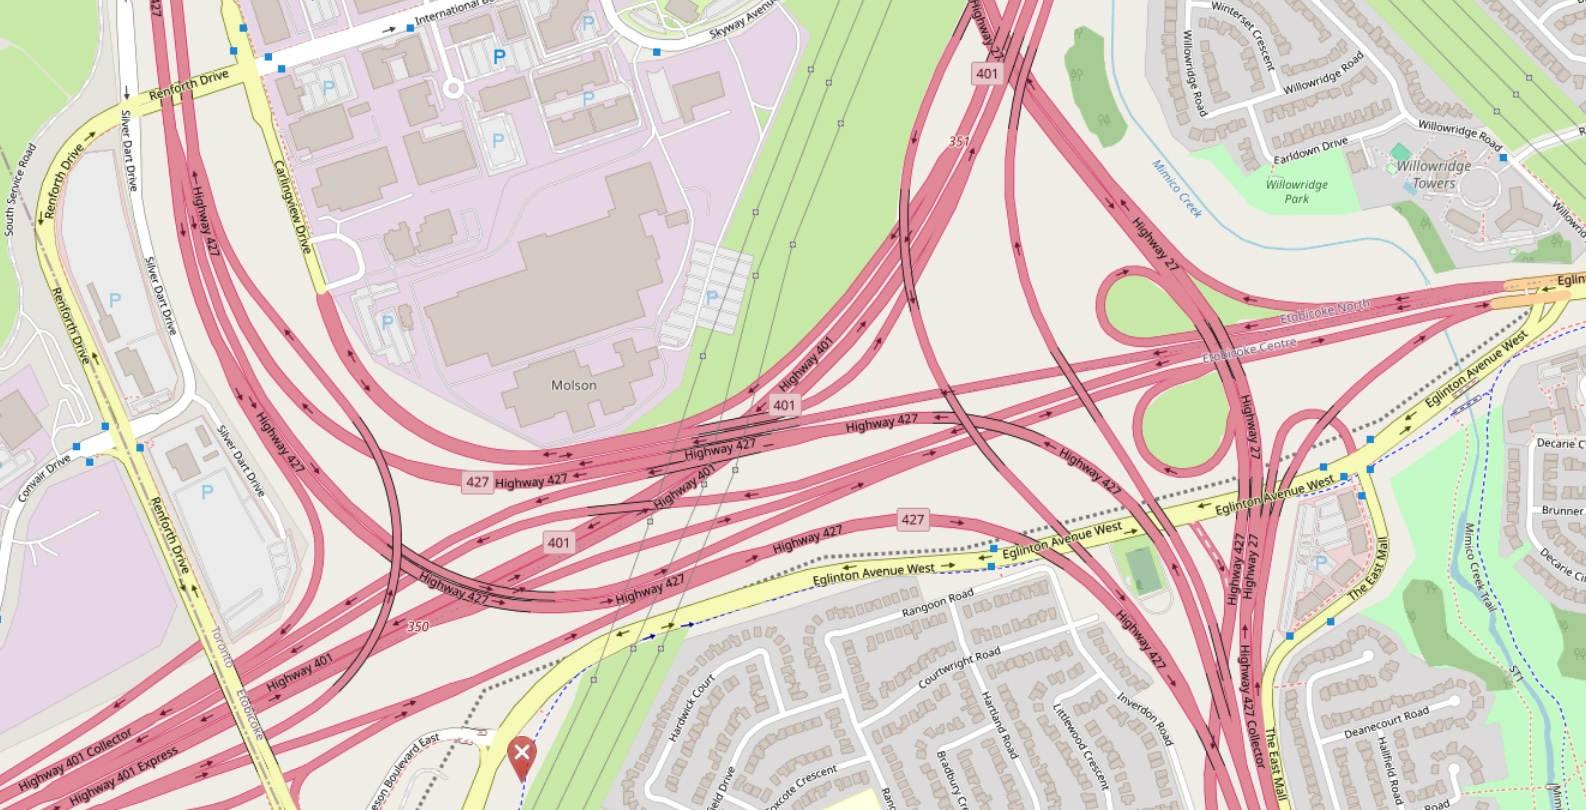
\includegraphics[width=0.8\textwidth]{figures/427map.jpg}
    \caption{The interchange complexity that results in a left-side exit from Hwy 427 southbound to Eglinton Avenue.}
    \label{fig:427map}
\end{figure}

We find similar adjustments for complexity in language. One is the so-called \textsc{heavy NP (Noun Phrase) shift}. A ``heavy'' NP is one with a lot of words in it: \textit{a book that I had found in a used-book store in Paris} is a heave NP, \textit{a book} is light. And the shift is a shift away from the verb, to the right in English, reflecting a ``short-before-long'' preference.

In heavy NP shift, the general ordering tendency is suppressed. The result, again, is to minimize the dependency distance between heads. In (\ref{ex:book-dep-dist-long}), we can count the number of words intervening between \textit{gave} and the head of each of the dependents (\textit{book}, \textit{to}, and \textit{for}) to find the dependency distance.

\ea \label{ex:book-dep-dist-long}
    \ea
        \begin{dependency}[theme = simple, arc angle=40]
           \begin{deptext}[column sep=0.1em, row sep=0.5cm]
              I \& gave \& a \& book \& to \& my \& best \& friend \& for \& Christmas.~~~$1+2+6=9$\\
           \end{deptext}
           \deproot[edge height=1.2cm]{2}{Head}
           \depedge[edge height=0.5cm]{2}{4}{1}
           \depedge[edge height=1cm]{2}{5}{2}
           \depedge[edge height=1.5cm]{2}{9}{6}
        \end{dependency}
    \ex[]{\textit{I gave \ob a \uline{book} that I had found in a used-book store in Paris\cb~\uline{to} my best friend \uline{for} Christmas.}\hfill$1+12+16=20$}
    \ex[]{\textit{I gave \uline{to} my best friend \uline{for} Christmas \ob a \uline{book} that I had found in a used-book store in Paris\cb.}\hfill$0+4+6=10$}\z
\z

The basic version in (a) has a total dependency distance of nine words. The (b) version is grammatical, but the heavy noun phrase in the basic sentences structure more than double the dependency distances. On the other hand, under the heavy NP shift, the dependency distance drops back to 10 words. Just as in the highway 427 exit example, there's a good reason to adjust the structure to accommodate unusual situation.

But if we try to do the same thing with a ``light'' NP (\ref{ex:light-NP-shift}), there's no justification, and so the unusual structure fails. It's ungrammatical. The shift is only allowed when there's a good reason for it.

\ea[*]{\textit{I gave to my best friend for Christmas \uline{a book}.} $0+4+6=10$}\label{ex:light-NP-shift}\z

The passive voice is another way to repackage things to reduce dependency distances. Consider the passive (\ref{ex:CNN}a) from Wikipedia with a dependency distance of zero between the underlined head of the subject and head verb. Now compare the active counterpart (b) with a dependency distance of 21.

\ea\label{ex:CNN}
    \ea[]{\textit{A convoluted neural network \uline{architecture} \uline{is} formed by a stack of distinct layers that transform the input volume into an output volume (e.g. holding the class scores) through a differentiable function.}\\\hfill[\textsc{passive}, 0]}
    \ex[]{\textit{A \uline{stack} of distinct layers that transform the input volume into an output volume (e.g. holding the class scores) through a differentiable function \uline{forms} a convoluted neural network architecture.}\hfill[\textsc{active}, 21]}\z
\z

\noindent No matter how many times you've been told to avoid the passive voice, I think you'll agree that the passive is better here.

One more example is illustrative here. Consider the difference between \textit{I threw out the trash} and \textit{I threw the trash out}. Both are fine, but as the \textit{trash} noun phrase becomes weighed down with more and more words in (\ref{ex:trash-out}), the pressure for the \textit{out}-first version builds. Notice the feeling of resolution going from (f) to (g).

\ea \label{ex:trash-out}
    \ea[]{\textit{I threw it out.}}
    \ex[]{\textit{I threw the trash out.}}
    \ex[]{\textit{I threw the kitchen trash out.}}
    \ex[]{\textit{I threw the smelly kitchen trash out.}}
    \ex[\textsuperscript{?}]{\textit{I threw the smelly kitchen trash from under the sink out.}}
    \ex[\textsuperscript{?}]{\textit{I threw the smelly kitchen trash from under the sink that had been sitting there for two weeks out.}}
    \ex[]{\textit{I threw out the smelly kitchen trash from under the sink that had been sitting there for two weeks.}}
    \z
\z

\begin{center}
-- --
\end{center}

\noindent As compact as a consistent head–dependent order is, 
%the one we've seen with verb + dependent (\textit{take a break}) and preposition + dependent (\textit{with a break}), 
there's a more efficient one. \citet{Gildea2007} show that alternating dependents minimizes dependency length. Under this ideal structure, a head with an even number of dependents would have one on each side. The odd dependents would still tend to the post-head position, at least in languages like English. This alternating-dependent structure is most effective at minimizing dependency distance in phrases with multiple dependents, such as verb phrases and noun phrases.

English turns out to be quite close to this ideal. Verb phrases mix head-before-dependent as in \textit{take a break} with dependent-before-head, as in \textit{I rested}. In the noun phrase, too, any determiner always precedes the noun -- we have \textit{the world}, \textit{this year}, \textit{some people}, \textit{many times}, \textit{my life}, and millions more.\footnote{By \textit{always}, I don't literally mean `always'. There are cases like \textit{I grant you wishes \uline{three}} or Shakespeare's \textit{o mistress \uline{mine}}.} But modifiers like relative clauses or preposition phrases typically follow the noun, as in \textit{the world \uline{that we live in}} or \textit{a person \uline{with knowledge of the changes}}.

Another factor is phrase length. If one dependent is pre-head and one post, which should go first? In a predominantly head-first language, like English, we've already seen that heavier -- that is longer -- phrases gravitate right. And the converse of that is that it is the shorter phrases that tend to occupy the pre-head positions.

You may have noticed that the determiner is a single word in all these examples, and typically a fairly short one at that. A determiner can be longer \textit{\uline{too many} people} or \textit{\uline{almost all} cases}, but almost all determiners are short, with the articles \textit{the} and \textit{a} dominating. The opposite holds for relative clauses (\textit{the things \uline{that he said}}) and preposition phrases (\textit{the girl \uline{with the green eyes}}). Shorter modifiers, like adjectives, tend to be pre-head (\textit{\uline{other} people}).


%\ea
%    \ea
%    \begin{dependency}[theme = simple]
%    \begin{deptext}[column sep=1em]
%    \textit{rest} \& \textit{the} \& \textit{of} \& \textit{us} \\
%    \end{deptext}
%    \deproot[edge height=0.5cm]{1}{Head}
%    \depedge{1}{2}{Det}
%    \depedge{1}{3}{Mod}
%    \depedge{3}{4}{Comp}
%    \end{dependency}
%    \ex
%    \begin{dependency}[theme = simple]
%    \begin{deptext}[column sep=1em]
%    \textit{the} \& \textit{rest} \& \textit{of} \& \textit{us} \\
%    \end{deptext}
%    \depedge{2}{1}{Det}
%    \deproot[edge height=0.5cm]{2}{Head}
%    \depedge{2}{3}{Mod}
%    \depedge{3}{4}{Comp}
%    \end{dependency}\z
%\z